%%%%%%%%%%%%%%%%%%%%%%% Boundary-Layer Meteorology 2019 Template %%%%%%%%%%%%%%%%%%%%%%%%%


% \begin{filecontents*}{example.eps}
% gsave
% newpath
%   20 20 moveto
%   20 220 lineto
%   220 220 lineto
%   220 20 lineto
% closepath
% 2 setlinewidth
% gsave
%   .4 setgray fill
% grestore
% stroke
% grestore
% \end{filecontents*}

\RequirePackage{fix-cm}
\documentclass[smallextended]{svjour3}
\smartqed
\usepackage{appendix}
\usepackage{amsmath,amssymb}
\usepackage{graphicx}
\usepackage{lineno}
\usepackage{array}
\usepackage{longtable}
\usepackage{natbib}
\setcitestyle{aysep={}}
\linenumbers

\newcommand*\patchAmsMathEnvironmentForLineno[1]{%
\expandafter\let\csname old#1\expandafter\endcsname\csname #1\endcsname
\expandafter\let\csname oldend#1\expandafter\endcsname\csname end#1\endcsname
\renewenvironment{#1}%
{\linenomath\csname old#1\endcsname}%
{\csname oldend#1\endcsname\endlinenomath}}%
\newcommand*\patchBothAmsMathEnvironmentsForLineno[1]{%
\patchAmsMathEnvironmentForLineno{#1}%
\patchAmsMathEnvironmentForLineno{#1*}}%
\AtBeginDocument{%
\patchBothAmsMathEnvironmentsForLineno{equation}%
\patchBothAmsMathEnvironmentsForLineno{align}%
\patchBothAmsMathEnvironmentsForLineno{flalign}%
\patchBothAmsMathEnvironmentsForLineno{alignat}%
\patchBothAmsMathEnvironmentsForLineno{gather}%
\patchBothAmsMathEnvironmentsForLineno{multline}%
}

\usepackage[dvipsnames]{xcolor}
\newcommand{\cg}{\textcolor{WildStrawberry}}


\begin{document}

\title{Local wind regime induced by the presence of giant linear dunes.}

\author{Cyril Gadal \and Pauline Delorme \and Clément Narteau \and
        Giles F.S. Wiggs \and Matthew Baddock \and Joanna M. Nield \and Philippe Claudin}

\institute{C. Gadal \at
              Institut de Mécanique des Fluides de Toulouse (IMFT), Université de Toulouse, CNRS, INPT, UPS, Toulouse, France \\
              \email{cyril.gadal@imft.fr}
           \and
           S. Author \at
              second address
            \and
            T. Author \at
            third address
}

\date{Received: DD Month YEAR / Accepted: DD Month YEAR}

\maketitle

\begin{abstract}
  In large-scale studies of arid areas, sediment fluxes and resulting geomorphological quantities (sediment pathways, erosion rates, dune morphodynamics) are often derived from wind data.
  %
  However, the feedback of nearby topography on the flow, such as kilometric giant dunes, is rarely taken into account because barely studied.
  %
  Here, we compare locally measured wind data to the predictions of the Era5Land climate reanalysis in four different places across and around the Namib sand sea. In places with flat environments, we show that the two wind datasets agree with each other. In contrast, within the sand sea, we show that they significantly differ due to the presence of giant linear dunes. We quantify this discrepancy, and link it to dynamics of the atmospheric boundary layer.
  %
  Aside setting limits to the applicability of the Era5land dataset, this study highlights the giant dunes feedback on the wind, and discuss its implications for smaller scale bedforms.
  %
  All codes used, from the raw data to the figures of the paper, are publicly available with full documentation at https://github.com/Cgadal/GiantDunes (will be made public upon acceptance of this manuscript for publication).

  \keywords{Boundary layer \and Turbulent flow \and Sand dunes \and Fluide-structures interactions}
\end{abstract}

\newpage

\section{Introduction}

As a flow encounters an obstacle, different interactions can arise depending on the different time and length scales involved. In the case of atmospheric flows, this mainly depends on the part of the atmosphere, schematically composed of a turbulent boundary layer topped by a stably stratified one, with which the obstacle interacts \citep{Stull1988}.
%
At the largest scale, the feedback of mountains on the stratified part results in wave generation as well as significant wind disturbances, such as downslope winds in the lee side \citep{Duran1990}. Inside the boundary layer, the interaction between a turbulent flow and hilly surfaces is for example key to the understanding ocean surface wind-driven waves~\citep{Sullivan2010}, or eolian bedforms in desert \citep{Courrech2015}.

Looking at the flow close to the surface, two different components of the topography feedback can be isolated. First, the flow accelerates on the upwind slope, and slows down on the downwind one, with a maximum velocity slightly upwind of the crest~\citep{Jackson1975, Sykes1980, Hunt1988}. Several measurements are available, performed in subaqueous flumes~\citep{Zilker1977, Zilker1979, Frederick1988} and in eolian field conditions~\citep{Claudin2013, Lu2021}. Second, deflection occurs when the incident flow direction is not perpendicular to the ridge crest. While predicted to be small (less than $10^{\circ}$) in the linear regime~\citep{Gadal2019}, significant flow steering has been reported in the field on the downwind side of larger aspect ratios obstacles, such as mountain ranges~\citep{Kim2000, Lewis2008, Fernando2019} or sand dunes~\citep{Walker2009, Walker2013, Hesp2015, Smith2017}.

In the case of aeolian bedforms, the measurements mentioned above were made on dunes a few meters high only. The resulting wind disturbances have then been shown to significantly impact the sediment pathways of the system \citep{Hesp2015}, but also to affect the collective behaviour of dune populations trough long-range interactions \citep{Bacik2020}.
%
However, eolian dunes coexists in sand seas at different scales, each representative of their different evolution stages, from emergence at twenty meters wavelengths to giant size, corresponding to kilometric wavelengths and heights of several dozen meters \citep{McKee1979}. Quantifying these two effects for giant dunes is then all the more important for several reasons.
%
First, larger wind disturbances are expected from larger obstacles.
%
Second, the flow--structure coupling is not straightforward due to vertical structure of the atmosphere with which the giant dunes interact due to their sizes \citep{andreotti2009}.
%
Finally, the morphodynamics of aeolian bedforms are strongly dependent on the wind regime~\citep{Livingstone1996}. Thus, small-scale bedforms are sensitive to wind disturbances induced by larger-scale bedforms. This has been demonstrated for impact ripples on dunes \citep{Howard1977,Hood2021}, but has never been studied for medium-scale dunes near giant dunes.

In the literature, arid areas have been studied at the desert scale from climate reanalyses based on global atmospheric models \citep{Blumberg1996, Livingstone2010, Ashkenazy2012, Jolivet2021, Hu2021}, such as ERA-40, ERA-Interim or ERA-5 \citep{Uppala2005, Dee2011, Hersbach2020}. However, the spatial resolution (tens of kilometers) of these reanalyses implies average quantities that do not resolve the smaller scales, ranging from the study of individual dunes to the border of mountains \citep{Livingstone2010}. Lately, the release of ERA5-Land allow to push back this limitation by providing up to 70 years of hourly wind predictions at a 9~km spatial resolution \citep{munoz2021}. However, due to its recent nature, the applicability limitations of this dataset remain to be studied.

Here, we compare local wind speeds and directions measured in four different places across the Namib desert to the regional predictions of the ERA5-Land climate reanalysis. When the measurement stations are surrounded by a relatively flat environment, we show that local measurements and regional predictions agree with each other. On the contrary, in the sand sea, we show that they differ due to the presence of giant dunes. Furthermore, we link the magnitude of these discrepancies to the circadian cycle of the atmospheric boundary layer. Finally, we draw implications for smaller-scale eolian bedforms.


\section{Wind regimes across the Namib Sand Sea}

  We focus on four places across and nearby the Namib desert, highlighting different environments (see Fig.~\ref{Fig1}).
  %
  The Adamax station is located near the Adamax salt pan, in a highly vegetated area. The Huab station, on the coast at the outlet of the Huab river, is in an arid environment exhibiting $60$-m scale barchan dunes. While the surroundings of these two stations are relatively flat, this is not the case for the Deep Sea and South Namib stations. Both are in the interdune between tens of meters high giant linear dunes with kilometric wavelengths and superimposed patterns. In this section, we describe and compare winds from local measurements and climate reanalysis predictions.

  \begin{figure}
    \centering
    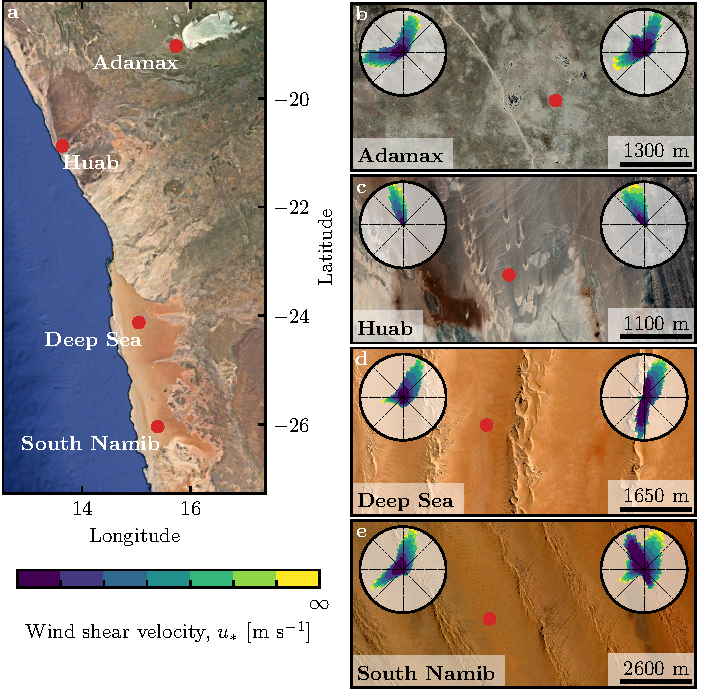
\includegraphics[scale=1]{Figures/Figure1.pdf}
    \caption{Wind data used in this study \textbf{a}: Location of the studied sites. \textbf{b--e}: Satellite images of the studied sites (Google-Earth, Maxar Technologies, CNES/Airbus). In each subplot, the left and right wind roses represent the data from the ERA5Land climate reanalysis and the local wind stations, respectively. Note that the bars show the direction towards which the wind blows. The black dots show the location of local wind stations.}
    \label{Fig1}
  \end{figure}

  \subsection{Datasets}

  Local winds are provided by measurement stations located in the four different places (see black dots in Fig.~\ref{Fig1}). The wind strength and direction are sampled every 10 minutes by cup anemometers and wind vanes, at heights between $2$~m and $3$~m depending on the station. The available period of measurements ranges from 1 to 5 discontinuous years distributed between 2012 and 2020 (see Fig.~\ref{Fig1_supp}). We checked that at least one complete seasonal cycle is available at each station.
  %
  Regional winds are extracted at the same locations and periods from the ERA5-Land dataset, which is a replay at a smaller spatial resolution of ERA5, the latest climate reanalysis from the ECMWWF \citep{Hersbach2020, munoz2021}. It provides hourly predictions of the 10-m wind velocity and direction at a spatial resolution of $\sim 9~\textup{km}$ ($0.1^\circ\times0.1^\circ$).


  For comparison, the local measurements are averaged into 1-hr bins centered on the temporal scale of the ERA5-Land estimates (see Fig.~\ref{Fig2_supp}). As the wind velocities of both datasets are provided at different heights, we convert them into shear velocities (see SI section 1), characteristic of the turbulent wind profile, which are then used together with the wind direction for further analysis. The resulting wind data are shown on the wind roses of Fig.~\ref{Fig1}(b--e).

  Finally, the dune properties are computed using autocorrelation on the 30-m Digital Elevation Models (DEMs) of the shuttle radar topography mission \citep{Farr2007}. For the South Namib and Deep Sea stations, we obtain respectively orientations of $85^\circ$ and $125^\circ$, wavelengths of $2.6~\textup{km}$ and $2.3~\textup{km}$ and amplitudes of $45~\textup{m}$ and $20~\textup{m}$ (see Fig.~\ref{Fig4_supp} for more details).

  \subsection{Agreement between local and regional winds}

  \begin{figure}
    \centering
    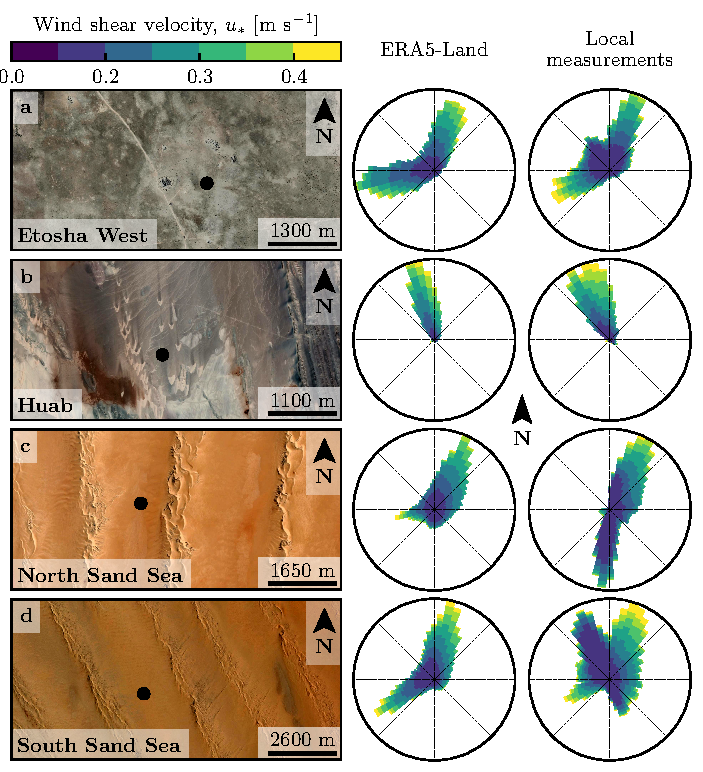
\includegraphics[scale=1]{Figures/Figure2.pdf}
    \caption{Temporal comparison between the wind data coming from the Era5Land climate reanalysis (orange lines) and from the local measurements (blue lines). Color swathes indicate day (between 1000 UTC and 2200 UTC) and night (before 1000 UTC or after 2200 UTC) \textbf{a--b}: Huab station. \textbf{c--d}: Deep Sea station in winter. \textbf{e--f}: Deep Sea station in summer.}
    \label{Fig2}
  \end{figure}

  The obtained wind regimes are shown in figure~\ref{Fig1}. In the Namib, the regional wind patterns are essentially controlled by the see breeze, resulting in strong northward components (sometimes slightly deviated by the large scale topography) present in all regional wind roses \citep{lancaster1985}. These daytime winds are dominant during the second-half of the year (Septembre-January). In winter, an additional easterly component can be recorded during the night, induced by the combination of katabatic winds forming on the mountains, and infrequent `berg' winds, which are responsible of the high wind velocities observed \citep{lancaster1984}. The frequency of these easterly components decreases from the inland to the coast, resulting in bidirectional wind regimes within the Namib Sand Sea and at the Adamax salt pan (Fig.~\ref{Fig1}b, \ref{Fig1}d and \ref{Fig1}e) and a unidirectional wind regime on the coast at the outlet of the Huab River (Fig.~\ref{Fig1}c).

  In the case of the Adamax and Huab stations, the wind roses from the regional predictions qualitatively match those corresponding to the local measurements. However, for the Deep Sea and South Namib stations, the measured wind roses exhibit additional components aligned with the giant dune orientation visible on the satellite images (Fig.~\ref{Fig1}c--d).
  %
  The time series of wind speed and direction show that this agreement in the case of Adamax and Huab stations is always verified (Fig.~\ref{Fig2}a--b) and Fig.~\ref{Fig5_supp}). In contrast, for the stations within the giant dune field, we observe that this agreement is limited to Septembre--January time periods (Fig.~\ref{Fig2}c--d).

  \subsection{Influence of the giant dunes on local wind regimes}
  \label{section_data_feedback}

  In the February--August period, when giant dunes are present, the local and regional winds match during daytime only, i.e when the southerly/southwesterly sea breeze dominates (see Fig.~\ref{Fig2}(e--f), Fig.~\ref{Fig3} and Fig.~\ref{Fig6_supp}). In the late afternoon and during the night, when the northwesterly `berg' and katabatic winds blow, measurements and predictions differ. In this case, the angular wind distribution of the local measurements exhibits two additional modes separated of $\simeq 180^\circ$, each corresponding to the giant dune alignement (see the purple frame in Fig.~\ref{Fig3} and Fig.~\ref{Fig6_supp}, as well as Fig.~\ref{Fig7_supp}). This deviation is also associated with a global attenuation of the wind strength (Fig.~\ref{Fig8_supp}). Remarkably, all these figures show that this process occurs for low wind velocities, typically for $u_{*} < 0.1~\textrm{m}~\textrm{s}^{-1}$. For shear velocities larger than $0.25~\textrm{m}~\textrm{s}^{-1}$, this wind reorientation does not occur. Finally, for intermediate shear velocities, both reorientation along the dune crest and no reorientation are observed (Fig.~\ref{Fig7_supp}).


  \begin{figure}
    \centering
    \includegraphics[scale=1]{Figures/Figure3.pdf}
    \caption{Distributions of wind direction at the Deep Sea Station for the Era5Land climate reanalysis (orange) and the local measurements (blue). In each subplot, both distributions are plotted from the same time steps, selected with constraints on the wind direction (columns) and/or wind velocity (rows) of the Era5Land dataset. The gray vertical dashed lines indicate the dune orientation. The numbers at the top right give the percentage of time steps selected in each sub-range, as well as the percentage of them corresponding to the day (between 1000 UTC and 2200 UTC). The purple frame highlights the regime (small wind velocities, nocturnal summer wind) in which the data from both datasets differs. A similar figure can be obtained for the Deep Sea station (see Fig.~\ref{Fig6_supp}).}
    \label{Fig3}
  \end{figure}


  \section{Influence of the circadian cycle of the atmospheric boundary layer}

  For linear ridges, dune-induced flow disturbances have mainly been related to the angle between wind direction and crest orientation, with a maximum for angles between $30^{\circ}$ and $70^{\circ}$~\citep{Walker2009, Hesp2015}. In our case, the most deflected wind for both stations is the most perpendicular, such that the incident wind direction does not seem to be the dominant parameter controlling the wind deflection. In contrast, a different behavior is observed between  low and high wind velocities, suggesting a change in hydrodynamical regime.

  In the following, we discuss the relevant parameters leading to different hydrodynamical interactions with topographical obstacles, and interpret the data with respect to the corresponding physical mechanisms.

  \begin{figure}
    \centering
    \includegraphics[scale=1]{Figures/Figure4.pdf}
    \caption{\textbf{a--b}: Vertical profiles of the virtual potential temperature at 2 different time steps (day - 31/03/2017 - 1200 UTC, night - 21/03/2017 - 2200 UTC) at the Deep Sea station. Dots: data from the ERA5 reanalysis. Transparent dashed lines: boundary layer height given by the ERA5 reanalysis, calculated from the bulk Richardson number \citep{seidel2012}. Plain lines: vertical (boundary layer) and linear (free atmosphere) fits to estimate the stratification properties. \textbf{c--f}: Sketches representing the interaction between the giant dunes and the atmospheric flow for different meteorological conditions. \textbf{g}: Streamlines qualitatively representing the effect of low, medium and high flow confinement. For details on the streamline derivation, see Appendix~\ref{turbulent_wind_model}.}
    \label{Fig4}
  \end{figure}

  \subsection{Relevant non-dimensional parameters and physical considerations}
  \label{theoretical_framework}

  Flow deflection over ridges can be understood from the Bernoulli principle~\citep{Hesp2015}. As the flow approaches the ridge crest, the compression of the streamlines results in larger flow velocities, and thus lower pressures~\citep{Rubin1987}. An incident flow oblique to the ridge is then deflected towards lower pressure zones, i.e towards the crest. Turbulent dissipation at the bottom and non-linearities tends to increase this effect downstream, resulting in along the crest wind deflection in the lee side~\citep{Hesp2015, Gadal2019}.

  Another way to increase the flow deflection is its confinement below a capping surface, that results in further streamline compression. This is the case for bedforms forming in open channel flows such as rivers~\citep{Fourriere2010, Unsworth2018}, but also for eolian dunes. These dunes evolve in the turbulent atmospheric boundary layer (ABL), which is capped by a transitional layer separating it from the stratified atmosphere above (see Fig.~\ref{Fig4}). Two different mechanisms control the possibility of this additional streamline compression.

  On one hand, it depends if the flow disturbance induced by the underlying topography reach the surface. As obstacles typically disturb flow over a characteristic height similar to their length, the potential of interaction between the dunes and the overlying surface is well captured by the parameter $k H$, where $k = 2\pi/\lambda$ is the wavenumber and $H$ the ABL depth. Note that $H$ is directly related to the radiative fluxes at the Earth surface, and thus varies with the circadian and seasonal cycles. Here, the giant dunes have kilometric wavelengths, such that $0.02 \lesssim k H \lesssim 5$, and they interact most of the time with the capping layer and the stratified free atmosphere (FA) above \citep{andreotti2009}. Interestingly, the limit of no-interactions between the topography and the boundary layer structure ($k H \gg 1$), in which the properties of the overlying atmospheric structure are irrelevant, is never reached here, in the case of giant dunes.

  On the other hand, it depends on rigidity of the capping surface, as its deformation releases the confinement effect inducing streamline compression. This is typically quantified using the Froude number~\citep{Vosper2004, Stull2006, Sheridan2006, Hunt2006, Jiang2014}:
  \begin{equation}
        \mathcal{F} = \displaystyle\frac{U}{\sqrt{\displaystyle\frac{\Delta\rho}{\rho_{0}}gH}},
  \end{equation}
  where $U$ is the wind velocity at the top of the ABL, $\rho_{0}$ its average density, $\Delta\rho$ the density jump between the ABL and the FA.


  % Note that the ability of the capping layer and stratification to accommodate a perturbation induced by the topography directly impacts the strength of this confinement effect (Fig.~\ref{Fig4}). This is typically quantified using surface and internal Froude numbers
  % \citep{Vosper2004, Stull2006, Sheridan2006, Hunt2006, Jiang2014}:
  % \begin{equation}
  %       \mathcal{F} = \displaystyle\frac{U}{\sqrt{\displaystyle\frac{\Delta\rho}{\rho}gH}}, \, \mathcal{F}_{\textup{I}} = \displaystyle\frac{k U}{N},
  % \end{equation}
  % where $U$ is the wind velocity at the top of the ABL, $\rho$ its average density, $\Delta\rho$ the density jump between the ABL and the FA and $N$ is the Brunt-Väisälä frequency, characteristic of the stratification.

  The smallest wind disturbances are expected during the day, when the ABL depth is comparable to the dune wavelength ($k H \gtrsim 1$) and for large wind velocities, which correspond to a weak confinement situation (Fig.~\ref{Fig4}d). On the contrary, large wind disturbances are expected to occur during the night, when the confinement is mainly induced by shallow ABL (Fig.~\ref{Fig4}e--f). Note that this strong confinement can be somewhat reduced in the case of strong winds (corresponding to large Froude numbers, see Fig.~\ref{Fig4}f), explaining the transition from deflected to non-deflected winds related to low and high velocities observed in the data (see section~\ref{section_data_feedback}).

  \subsection{Flow regime diagrams}

  To highlight these different regimes from our data, we compute wind disturbance diagrams in the space defined by the two relevant non-dimensional numbers presented above, $\left(k H,\, \mathcal{F}\right)$. Those are calculated from the time series of the geopotential, temperature and specific humidity vertical profiles available in the ERA5 climate reanalysis (see SI section 2).
  %
  Flow deviation is computed as the minimal angle between the wind orientations from the local measurements, and the regional predictions. The relative velocity modulation is computed as
  %
  \begin{equation}
    \delta_{\textup{u}} = \frac{u_{*}^{\textup{ERA}} -  u_{*}^{\textup{station}}}{u_{*}^{\textup{ERA}}}.
  \end{equation}

  When representing the two variables $\delta_{\theta}$ and $\delta_{\textup{u}}$ in this space, different regime emerges (Fig.~\ref{Fig5}). Small wind disturbances ($\delta_{\theta} \to 0$, $\delta_{\textup{u}} \to 0$) are located in the top-right part of the diagrams, corresponding to a regime mixing low-interaction and low-confinement ($k H$ and $\mathcal{F}$ large enough, Fig.~\ref{Fig4}d).
  %
  Lower values of $k H$ (stronger interaction) or Froude number (stronger confinement) then both lead to an increase in wind disturbances, both in terms of orientation and velocity. Below a threshold value of $k H \simeq 0.3$, wind disturbance occurs independently of the Froude number value, probably due to enhanced non-linear effects linked to strong flow modulation by the obstacle in this part of the diagram. The Froude number also controls a transition from damped to amplified wind velocities in the interdune, with a transition at $\mathcal{F} \simeq 0.4$ (Fig.~\ref{Fig5}b). This may be linked to a transition in the flow regime in the lee side of the obstacle (lee waves, hydraulic jumps, rotors) but further measurements are needed in order to assess this \citep{baines1995, Vosper2004}.

  %
  % Furthermore, this also seems to control a transition between from damped to amplified wind velocities within the interdune (Fig.~\ref{Fig5}b), for which we do not have an explanation. Note that the same interpretation can be done with the diagrams including the internal Froude number $\mathcal{F}_{\textup{I}}$, as shown by Fig.~\ref{Fig12_supp}.

  \begin{figure}
    \centering
    \includegraphics[scale=1]{Figures/Figure5.pdf}
    \caption{Regime diagrams of the wind deviation $\delta_{\theta}$ and relative attenuation/amplification $\delta_{u}$ in the space $(\mathcal{F}, \, kH)$, containing the data from both the Deep Sea and South Namib stations. Blue dashed lines empirically delimit the different regimes. The point density in each bin of the diagrams is shown in Fig.~\ref{Fig11_supp}. The regime diagrams in the spaces $(\mathcal{F}_{\textup{I}}, \, kH)$ and $(\mathcal{F}_{\textup{I}}, \, \mathcal{F})$ are shown in Fig.~\ref{Fig12_supp}.}
    \label{Fig5}
  \end{figure}

  \subsection{On the influence of the stratification of the free atmosphere}

  The presence of a stratification in the free atmosphere can also impact the flow confinement, depending on its ability to deform under the presence of an underlying obstacle. This can be quantified using the internal Froude number~\citep{Vosper2004, Stull2006, Sheridan2006, Hunt2006, Jiang2014}:
  \begin{equation}
    \mathcal{F}_{\textup{I}} = \displaystyle\frac{k U}{N},
  \end{equation}
  where $N = \sqrt{-(g/\rho_{0})(\partial \rho/\partial z)}$ is characteristic of the stratification. Both Froude numbers have the same qualitative effect on flow confinement, as they quantify the rigidity of the overlying layers. This is confirmed by figure~\ref{Fig12_supp}, where we can also find the different regimes related to wind disturbances described previously for the Froude number $\mathcal{F}$.

\section{Discussion}

  \begin{figure}
    \centering
    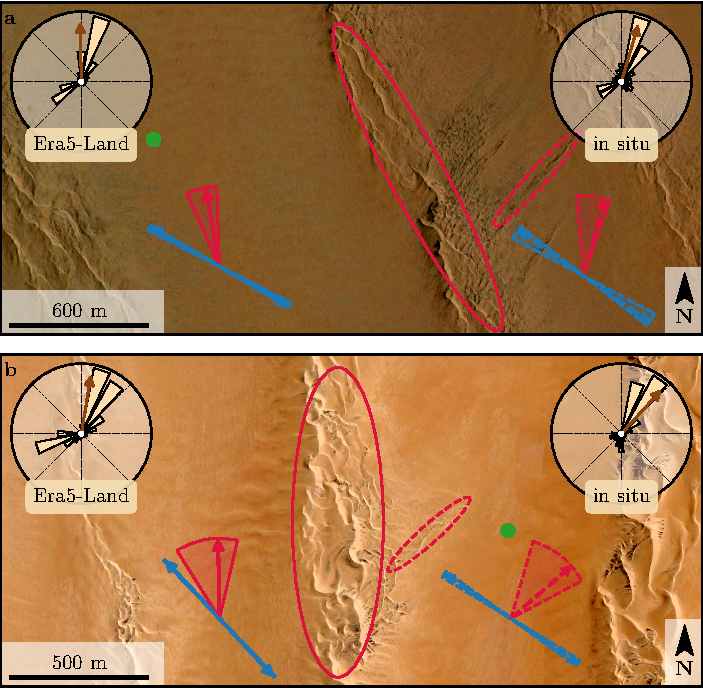
\includegraphics[scale=1]{Figures/Figure6.pdf}
    \caption{Implications for smaller scale patterns in (a) the South Namib and (b) Deep Sea. The ellipses indicates the diffe  rent types of elongating dunes, at large (plain) and small scale (dashed). The dune orientations are calculated using the model of \citet{Courrech2014} from the sand flux angular distributions, shown here for typical sand quartz grains of $180~\mu$m. The double blue and single red arrows correspond to the two possible dune growth mechanisms, bed instability and elongation, respectively. Likewise, plain arrows are calculated from the ERA5-Land data, and dashed arrows from the local measurements. Wedges show the uncertainty on the orientation calculation, and the arrows correspond to typical parameters found in the literature, i.e a grain diameter of $180~\mu$m and a flux-up ratio of 1.6. The black dots indicate the position of the measurement stations. See Appendix 2 for additional details.}
    \label{Fig6}
  \end{figure}

 The comparison of local (direct measurements) and regional (climate reanalysis) wind data reveals the giant dunes feedback on the flow. In flat areas, the matching between measurements and prediction confirms the ability of the ERA5Land climate reanalysis to predict the wind flow down to scales $\sim 10~\textrm{km}$, i.e the grid model. When smaller scale topographies are present (giant dunes in our case), locally measured wind regimes can significantly differ from the regionally predicted ones. Furthermore, we link these disturbances induced by the dunes to their interaction with the lower part of the atmospheric vertical structure, and more specifically to its circadian variability. During the night, the presence of a shallow atmospheric boundary layer (ABL) induces a strong confinement of the flow, associated with large wind deviation and acceleration or deceleration. During the day, the capping layer is high enough to prevent its interaction with the giant dunes, resulting in a low confinement of the flow, and thus smaller wind disturbances. Interestingly, we also found that this effect could be counterbalanced by the presence of large wind velocities, capable of deforming the capping layer and/or the FA stratification, thus decreasing the confinement effect.

 Simple linear models also suggest that larger wind disturbances occur under strong flow confinement such as described above \citet{andreotti2009, Andreotti2012}. However, they are unable to reproduce the magnitude of the observed deviations, probably due to the presence of hydrodynamical non-linear effects, all the more present in high confinement situations linked to strong flow modulations (see Fig.~\ref{Fig12_supp} and Appendix 1). They also predict different spatial flow structures such as lee waves and rotors~\citep{baines1995, Vosper2004}, which are likely to be complicated by these non-linearities, and which cannot be observed by our single point measurements. Measurements in different places along and across the ridge are then needed in order to properly map these flow structures, and allow further comparisons with models.

 This study highlights the interaction between giant dunes and the atmospheric boundary layer. It then supports the debated idea that the capping layer acts as a bounding surface limiting dune growth~\citep{andreotti2009}, as opposed to an unconstrained growth ever-slower with size \citep{Eastwood2011, gunn2021}. Once validated, this mechanism would then allow inference of the ABL depth from the giant bedforms spacing where measurements are not feasible or available, as performed by~\citet{Lorenz2010} on Titan.

 This interaction also have strong implications for smaller scales bedforms, as illustrated in Fig.~\ref{Fig6}. In the Namib Sand Sea, small linear dunes ($\sim 50$ m -wide) are present in the interdune between giant linear dunes ($\sim 2$ km -wide). While differences between larger and smaller scale dune patterns are observed ubiquitously, they are now largely attributed to the presence of two different dune growth mechanisms, leading to two different dune patterns (orientations and/or morphologies) for the same wind regime~\citep{Courrech2014, Runyon2017, lu2017, Song2019, Hu2021}. Here, coupling sediment transport and dune growth models, we show that the orientations of the small and giant linear dunes can be predicted from the same dune growth mechanism, using the locally measured and regionally predicted winds, respectively (red arrows in Fig.~\ref{Fig6}). The giant dune feedback on the flow described in this study then provides a mechanism for the existence of these small linear dunes elongating across the interdune, as yet unresolved. While further studies are needed, these dune type could provide additional strong constraints for the inference of local winds from bedforms, as currently performed on Mars using ripple orientations \citep{Liu2015, Hood2021}.


\begin{acknowledgements}
We would like to acknowledge the contributors of the following open-source python librairies, Matplotlib \citep{Hunter2007}, Numpy \citep{Harris2020} and Scipy \citep{Virtanen2020}, which provide an incredibly efficient ecosystem allowing scientific research in Python.

Era5 and Era5Land datasets are publicly available at the Copernicus Climate Change Service (C3S) Climate Data Store. The locally measured wind data can be found at \cg{upload on public data repository}. The digital elevation models from the Shuttle Radar Topography Mission are publicly available from Nasa servers, and can be downloaded at https://dwtkns.com/srtm30m/. Fully documented codes used to analyze this study are available at https://github.com/Cgadal/GiantDunes (will be made public upon acceptance of this manuscript for publication).

[citing all grants ...]\\
\end{acknowledgements}

\section*{Appendix 1: ABL turbulent wind model}
\label{turbulent_wind_model}

Following the work of \citet{Fourriere2010}, \citet{Andreotti2012} anc \citet{andreotti2009}, we briefly expose in this section the linear response of a turbulent flow to a small aspect ratio perturbation of the underlying topography. As this topography can be decomposed into several sinusoidal modes, we focus on a sinusoidal topography:
\begin{equation}
  \xi = \xi_{0}\cos\left[k\left(\cos(\alpha)x + \sin(\alpha)y\right)\right],
\end{equation}
which is also a good approximation for the giant dunes observed in the Deep Sea and South Namib Station (see Fig~\ref{Fig1} and Fig~\ref{Fig4_supp}). Here, $x$ and $y$ are the streamwise and spanwise coordinates, $k=2\pi/\lambda$ the wavenumber of the sinusoidal perturbation, and $\alpha$ its crest orientation, calculated with respect to the $y$--direction.

The two components of the basal shear stress $\boldsymbol{\tau} = \rho_{0} u_{*}\boldsymbol{u}_{*}$, constant in a flat bottom situation, can then be written without loss of generality as:
\begin{align}
  \tau_{x} & = \tau_{0}\left(1 + k\xi_{0}\sqrt{\mathcal{A}_{x}^{2} + \mathcal{B}_{x}^{2}}\cos\left[k\left(\cos(\alpha)x + \sin(\alpha)y\right) + \phi_{x}\right]\right), \\
  \tau_{y} & = \tau_{0}k\xi_{0}\sqrt{\mathcal{A}_{y}^{2} + \mathcal{B}_{y}^{2}}\cos\left[k\left(\cos(\alpha)x + \sin(\alpha)y\right) + \phi_{y}\right],
\end{align}
where $\tau_{0}$ is the basal shear stress on a flat bed, and $\phi_{x, y} = \tan^{-1}\left(\mathcal{B}_{x, y}/\mathcal{A}_{x, y}\right)$. The in--phase and in--quadrature hydrodynamical coefficients $\mathcal{A}_{x, y}$ and $\mathcal{B}_{x, y}$ are functions of the flow conditions, i.e the bottom roughness, the vertical flow structure or the incident flow direction \citep{Fourriere2010, andreotti2009, Andreotti2012}.

Following \citet{Andreotti2012}, the impact of the incident wind direction can be approximated by the following expressions:
\begin{align}
  \mathcal{A}_{x} & = \mathcal{A}_{0}\cos^{2}\alpha, \\
  \mathcal{B}_{x} & = \mathcal{B}_{0}\cos^{2}\alpha, \\
  \mathcal{A}_{y} & = \displaystyle\frac{1}{2}\mathcal{A}_{0}\cos\alpha \sin\alpha, \\
  \mathcal{B}_{y} & = \displaystyle\frac{1}{2}\mathcal{B}_{0}\cos\alpha \sin\alpha,
\end{align}
where $\mathcal{A}_{0}$ and $\mathcal{B}_{0}$ are now two coefficients independent of the dune orientation $\alpha$. In the case of a fully turbulent boundary layer capped by a stratified atmosphere, they now only depend on $k H$, $k z_{0}$, $\mathcal{F}$ and $\mathcal{F}_{\textup{I}}$ \citet{andreotti2009}. In this study, we assume a constant hydrodynamic roughness $z_{0} \sim 1~\textup{mm}$, leading to a constant value of $k z_{0} \sim 10^{-6}$. Measured values of $z_{0}$ in the field indeed reports a variation of $z_{0}$ between 0.1 mm and 10 mm \citep{Sherman2008, Field2018}, but $\mathcal{A}_{0}$ and $\mathcal{B}_{0}$ does not vary much in the corresponding range of $k z_{0}$ \citep{Fourriere2010}.
%
Note that the linearity assumption of this theoretical framework requires $\left(\vert \tau \vert - \tau_{0}\right)/\tau_{0} \ll 1$, which is satisfied by $k\xi\sqrt{\mathcal{A}_{0}^{2} + \mathcal{B}_{0}^{2}} \ll 1$. In our case, the giant dune morphology gives $k\xi \simeq 0.1$, setting the upper bound of the coefficient modulus $\sqrt{\mathcal{A}_{0}^{2} + \mathcal{B}_{0}^{2}}$ to 10.


Additionlly, we also calculate the time series of the hydrodyamical coefficients from the time series of the non-dimensional numbers used in this study. The results, shown Fig.~\ref{Fig12_supp} under the similar form of the regime diagrams presented in Fig.~\ref{Fig5} and Fig.~\ref{Fig12_supp}, exhibit a qualitative matching with the observations presented in this study.
%
Small values of these coefficients ($\mathcal{A}_{0} \simeq 3.4$ and $\mathcal{B}_{0} \simeq 1$) are found in low confinement cases, i.e for $k H \gg 1$ (no interaction between the dunes and the capping layer) or for $k H \gg 1$ but large enough Froude numbers (reduced flow confinement due to the deformation of the olverlying capping layer and stratification). In contrast, larger values are obtained in high confinement cases (small $k H$ and Froude numbers). However, not that most of this part of the diagrams are outside of the linear limit discussed above ($\sqrt{\mathcal{A}_{0}^{2} + \mathcal{B}_{0}^{2}} \gtrsim 10$), which does not allow further quantitative comparison with the data.


\section*{Appendix 2: Sediment transport and dune morphodynamics}

Here, we briefly describe the sediment transport and dune morphodynamics theoretical framework leading to the prediction of sand fluxes and dune orientations from wind data.

\paragraph{Sediment transport}
The prediction of sand fluxes from wind data has been a long standing issue in geomorphological studies~\citep{Fryberger79, Pearce2005, Sherman2012, Shen2019}. Based on laboratory studies in wind tunnels \citep{Rasmussen96, Iversen99, Creyssels2009, Ho2011}, as well as physical considerations \citep{Ungar1987, Andreotti2004bis, Duran2011, Pahtz2020}, it has been shown that the steady saturated sand flux over a flat sand bed depends linearly on the shear stress:
\begin{equation}
  \label{transport_law_quadratic}
  \frac{q_{\textup{sat, t}}}{Q} = \Omega\sqrt{\Theta_{\textup{th}}}\left(\Theta_{t} - \Theta_{\textup{th}}\right),
\end{equation}
where $\Omega$ is a proportionality constant, $Q = d\sqrt{(\rho_{\textup{s}} - \rho_{0})gd/\rho_{0}}$ is a characteristic flux, $\Theta = \rho_{0} u_{*, t}^{2}/(\rho_{\textup{s}} - \rho_{0})gd$ the Shields number, and $\Theta_{\textup{th}}$ its threshold value for incipient sediment transport. Here, $\rho_{\textup{s}} = 2.6~\textup{g}~\textup{cm}^{-3}$ and $d=180~\mu\textup{m}$ are the grain density and diameter, and $g$ is the gravitational acceleration.

Recently, \citet{Pahtz2020} suggested a quadratic dependency on the shear stress by taking into account grain--grain interactions within the transport layer, performing better at reproducing laboratory data at high wind velocities:
\begin{equation}
  \label{transport_law_quartic}
  \frac{q_{\textup{sat, t}}}{Q} = \frac{2\sqrt{\Theta_{\textup{th}}}}{\kappa\mu}\left(\Theta_{t} - \Theta_{\textup{th}}\right)\left(1 +\frac{C_{\textup{M}}}{\mu}\left[\Theta_{t} - \Theta_{\textup{th}}\right]\right),
\end{equation}
where $\kappa = 0.4$ is the von Kármán constant, $C_{\rm M}=1.7$ a constant and $\mu$ a friction coefficient, taken to be the avalanche slope of the granular material, i.e $\sim 0.6$. The fit of this law to the experimental data of \citet{Creyssels2009} and \citet{Ho2011} gives $\Theta_{\textup{th}} = 0.0035$. The sand flux angular distributions and the dune orientations in Fig.~\ref{Fig6} are calculated using this quartic law \eqref{transport_law_quartic}. However, we verified that using the quadratic law \eqref{transport_law_quadratic} instead did not change the predicted dune orientations by more than a few degrees.

\paragraph{Dune orientations}

The dune orientations are predicted from the computed sand flux time series, using the dimensional model of \citet{Courrech2014}. Two orientations are possible depending on the mechanism dominating the dune growth: elongation or bed instability (the latter is also known as the rule of maximum gross bedform-normal transport from \citet{Rubin1987}).

The orientation $\alpha$ corresponding the bed instability is then the one that maximizes the following growth rate:
\begin{equation}
  \sigma \propto \frac{1}{H_{d} W_{d} T}\int_{t}  q_{\textup{crest}, t}\vert \sin\left(\theta_{t} - \alpha\right) \vert,
\end{equation}
where $H_{d}$ and $W_{d}$ are dimensional constants representing the dune height and width, respectively. The flux at the crest is expressed as:
\begin{equation}
  q_{\textup{crest}, t} = q_{\textup{sat}, t}\left[1 + \gamma\vert\sin\left(\theta_{t} - \alpha\right)\vert\right],
\end{equation}
where the flux-up ratio $\gamma$ has been calibrated to 1.6 using field studies, underwater laboratory experiments and numerical simulations. Similarly, the dune orientation corresponding to the elongation mechanism is the one that verifies:
\begin{equation}
  \tan(\alpha) = \frac{\langle q_{\textup{crest}, t}(\alpha) \boldsymbol{e}_{\theta_{t}}\rangle \cdot \boldsymbol{e}_{WE} }{ \langle q_{\textup{crest}, t}(\alpha) \boldsymbol{e}_{\theta_{t}} \rangle \cdot \boldsymbol{e}_{SN}},
\end{equation}
where $\langle.\rangle$ denotes a vectorial time average. The unitary vectors $\boldsymbol{e}_{WE}$, $\boldsymbol{e}_{SN}$ and $\boldsymbol{e}_{\theta_{t}}$ are in the West--East, South--North and wind direction, respectively.

The resulting computed dune orientations, blue and red arrows in figure~\ref{Fig6}, are then depending on a certain number of parameters (grain properties, flux-up ratio), for which we took typical values for eolian desert on Earth. Due to the lack of measurements in the studied places, significant uncertainties can however be expected. We therefore run a sensibility test by calculating the dune orientations for grain diameters ranging from $100~\mu\textup{m}$ to $400~\mu\textup{m}$ and the speed-up ratio from $0.1$ to $10$ (wedges on figure~\ref{Fig6}).

\clearpage

\bibliographystyle{spbasic_updated}
\bibliography{biblio}

\newpage
\renewcommand{\thefigure}{S\arabic{figure}}
\setcounter{figure}{0}

\section*{Supplementary Material for \textit{Boundary-Layer Meteorology} Sample Paper: Instructions for Authors}

{\textbf{First Author* $\cdot$ Second Author $\cdot$ Third Author \\}}
\\
\text{*}Affiliation and email address for the corresponding author only (note that the corresponding author does not need to be the first author).

\begin{figure}
  \centering
  \includegraphics[scale=1]{Figures/Figure1_supp.pdf}
  \caption{Gant chart representing the valid time steps for the two data sets, for all stations.}
  \label{Fig1_supp}
\end{figure}

\begin{figure}
  \centering
  \includegraphics[scale=1]{Figures/Figure2_supp.pdf}
  \caption{Comparison between raw local wind measurements, and centered averaged data over one hour for the South Namib station. \textbf{a}: wind direction. \textbf{b}: wind velocity at the measurement height, 2.6 m.}
  \label{Fig2_supp}
\end{figure}

\section*{1. Shear velocity and calibration of the hydrodynamical roughness}
\label{calib_z0}

As the regionally predicted and locally measured velocities are available at different heights, we can not compare them directly. We then convert all velocities into shear velocities $u_{*}$, characteristic of the turbulent velocity profile \citep{Spalding1961, Stull1988}:
\begin{equation}
  \frac{u(z)}{u_{*}} = \frac{1}{\kappa}\ln\left(\frac{z}{z_{0}}\right),
\end{equation}
where $z$ is the vertical coordinate, $\kappa \approx 0.4$ the von Kármán constant and $z_{0}$ the hydrodynamic roughness. Several field measurements of hydrodynamic roughnesses are available. In the absence of sediment transport, it scales with the geometric roughness of the topography \citep{Pelletier2016}. When transport occurs, it then scales with the thickness of the transport layer ($\sim 1$~mm), depending on the wind velocity and grain properties \citep{Sherman2008, Zhang2016, Field2018}.

The different environments of our stations (vegetated, arid, sandy) makes it difficult to develop a precise model for the computation of the hydrodyamic roughness. Furthermore, we do not have precise enough topographical measurements that would allow to compute the geometric roughness. We choose to leave aside this complexity, and use a different approach. The selected hydrodynamic roughness is then the one that leads to the best possible matching between the regionally predicted and locally measured winds.


For each station, the hydrodynamic roughness is calibrated by finding the one that minimizes the relative difference $\delta$ between the wind vectors of both datasets:
\begin{equation}
  \label{metric_roughness}
      \delta = \frac{\sqrt{\langle\| \boldsymbol{u}_{*, \textrm{era}} - \boldsymbol{u}_{*, \textrm{station}} \|^{2}\rangle_{t}}}{\sqrt{ \langle \| \boldsymbol{u}_{*, \textrm{era}} \| \rangle_{t}\langle \| \boldsymbol{u}_{*, \textrm{station}} \| \rangle_{t}}}
\end{equation}
This $\delta$--parameter is computed for hydrodynamic roughness values ranging from $10^{-5}$~m to $10^{-2}$~m for the different stations. Note that for the Deep Sea and South Namib stations, where the giant dunes feedback presumably affect the wind, we take into account the non-deflected winds only in the calculation of $\delta$ (with a $15\circ$ tolerance).


A shown by figure~\ref{Fig3_supp}, the minimum of $\delta$ in the space ($z_{0}^{\textup{Era5Land}}$, $z_{0}^{\textup{local}}$) forms a line. We thus take the roughness of the Era5Land dataset as the typical value when sediment transport occurs, $10^{-3}$~m, corresponding to the thickness of the transport layer \citep{Duran2011}. It leads for the Adamax, Deep Sea, Huab and South Namib stations values of $2.7~\textup{mm}$, $0.76~\textup{mm}$, $0.12~\textup{mm}$ and $0.48~\textup{mm}$, respectively.

The choice of the hydrodynamic roughness values impacts the calculated shear velocities only, but not the wind directions. As such, most of our conclusions are independent of such a choice. However, it may affect the magnitude of the wind velocity attenuation/amplification in flow confinement situations.


\begin{figure}
  \centering
  \includegraphics[scale=1]{Figures/Figure3_supp.pdf}
  \caption{Calibration of the hydrodynamic roughnesses. The metric $\delta$ defined in \eqref{metric_roughness} is represented in colorscale as a function of the hydrodynamic roughnesses chosen for the Era5-Land and local winds, for the (\textbf{a}) Adamax, (\textbf{b}) Deep Sea, (\textbf{c}) Huab and (\textbf{d}) South Namib stations. The red dashed and plain lines shows the minima of $\delta$ and the identity line, respectively. The orange lines and dots highlight the chosen hydrodynamic roughnesses for the local winds, by imposing $z_{0}^{\textup{Era5Land}} = 1~\textup{mm}$. It leads for for each station to $2.7~\textup{mm}$, $0.76~\textup{mm}$, $0.12~\textup{mm}$ and $0.48~\textup{mm}$, respectively.}
  \label{Fig3_supp}
\end{figure}


\begin{figure}
  \centering
  \includegraphics[scale=1]{Figures/Figure4_supp.pdf}
  \caption{Analysis of the DEMs of the Deep Sea (left column -- \textbf{a}, \textbf{b}, \textbf{c}) and South Namib (right column -- \textbf{d}, \textbf{e}, \textbf{f}) stations. \textbf{a--d}: Detrended topography (a second order polynomial is first fitted and then removed) . \textbf{b--e}: autocorrelation matrix shown in colorscale. The black line shows the detected orientation, and the red line the profile along which the wavelength is calculated, shown in \textbf{c--f}. The blue lines and dots show the first peak of the autocorrelation profile, whose abscissa gives the characteristic wavelength of the dune pattern.}
  \label{Fig4_supp}
\end{figure}

\begin{figure}
  \centering
  \includegraphics[scale=1]{Figures/Figure5_supp.pdf}
  \caption{Statistical agreement of the wind orientation (\textbf{a}) and velocity (\textbf{b}) between the Era5Land dataset and the local measurements for the Huab and Adamax stations. Note how the points are clustered around identity lines (dashed and black).}
  \label{Fig5_supp}
\end{figure}

\begin{figure}
  \centering
  \includegraphics[scale=1]{Figures/Figure6_supp.pdf}
  \caption{Distributions of wind direction at the South Namib Station for the Era5Land climate reanalysis (orange) and the local measurements (blue). In each subplot, both distributions are plotted from the same time steps, selected with constraints on the wind direction (columns) and/or wind velocity (rows) in the Era5Land dataset. The gray vertical dashed lines indicate the dune orientation. The numbers at the top center give the percentage of time steps selected in each sub-range, as well as the percentage of them corresponding to the day (between 1000 UTC and 2200 UTC). The purple frame highlights the regime (small wind velocities, nocturnal summer wind) during which the wind data from both datasets differs. A similar figure can be obtained for the South Namib station (see Fig.~\ref{Fig3}).}
  \label{Fig6_supp}
\end{figure}

\begin{figure}
  \centering
  \includegraphics[scale=1]{Figures/Figure7_supp.pdf}
  \caption{Statistical comparison of the wind orientation between the Era5Land dataset and the local measurements for the South Namib and Deep Sea stations, for different velocity ranges. \textbf{a}: $u_{*, \textup{\textup{ERA}}} < 0.1~\textup{m}~\textup{s}^{-1}$. \textbf{b}: $0.1 < u_{*, \textup{\textup{ERA}}} \leq 0.25~\textup{m}~\textup{s}^{-1}$. \textbf{c}: $u_{*, \textup{\textup{ERA}}} \geq 0.25~\textup{m}~\textup{s}^{-1}$. Note that the measured dune orientations are substracted to the wind orientation, which allows to plot both stations on the same graph. Black dashed lines indicate locally measured orientations aligned with the dune crests (here $0^\circ$, $180^\circ$ and $360^\circ$ -- \textbf{a}, \textbf{b}), as well as the identity lines (\textbf{b}, \textbf{c}).}
  \label{Fig7_supp}
\end{figure}

\begin{figure}
  \centering
  \includegraphics[scale=1]{Figures/Figure8_supp.pdf}
  \caption{Statistical comparison of the wind velocity between the Era5Land dataset and the local measurements for the South Namib and Deep Sea stations. \textbf{a}: Nocturnal summer easterly wind. \textbf{b}: Diurnal southerly wind. Black dashed lines are identity lines. The angle ranges used to select diurnal and nocturnal summer winds are those taken in Fig.~\ref{Fig3} and Fig.~\ref{Fig6_supp}.}
  \label{Fig8_supp}
\end{figure}

\section*{2. Extraction of the ABL properties}

The estimation of the non-dimensional numbers requires the computation of meteorological quantities representative of the current atmospheric boundary layer. In arid areas, the vertical structure of the atmosphere can be approximated by well mixed convective boundary layer of height $H$, topped by the stratified free atmosphere \citep{Stull1988, Shao2008}.
%
In this type of structure, the virtual potential temperature is constant inside the boundary layer, and then increases linearly in the stratified free atmosphere (Fig.~\ref{Fig9_supp}a):
\begin{equation}
  T_{\textup{vp}}(z) = \begin{cases}
                          T_{0} &\text{for $z < H$},\\
                          T_{0}\left(1 + \displaystyle\frac{\Delta T_{\textup{vp}}}{T_{0}} + \frac{N^{2}}{g}(z - H)\right) &\text{for $ z > H$},
                        \end{cases}
\end{equation}
where, $T_{0}$ is the surface virtual potential temperature, $\Delta T_{\textup{vp}}$ the discontinuity at the capping layer and $N$ the Brunt-Väisälä frequency, characteristic of the stratification.

The Era5 dataset provides a direct estimate of the ABL depth $H$ from a bulk Richardson number calculation, as well as vertical profiles of the geopotential $\phi$, temperature $T$ and specific humidity $e_{\textup{w}}$ at given pressure levels $P$. From these quantities, the virtual potential temperature can be calculated as:
\begin{equation}
  T_{\textup{vp}} = T\left(1 + \left[R_{\textup{M}} - 1\right]e_{\textup{w}}\right)\left(\frac{P_{0}}{P}\right)^{P_{\textup{c}}(1 - 0.24e_{\textup{w}})},
\end{equation}
where $P_{0} = 10^{5}~\textup{Pa}$ is the standard pressure, $P_{\textup{c}} = 0.2854$ the Poisson coefficient for dry air and $R_{\textup{M}}=1.61$ is the ratio between the molecular masses of dry air and water. The vertical coordinates are calculated as:
\begin{equation}
  z = \frac{\phi R_{\textup{t}}}{g R_{\textup{t}} - \phi},
\end{equation}
where $R_{\textup{t}} = 6356766~\textup{m}$ is the average Earth radius, and $g = 9.81~\textup{m}~\textup{s}^{-2}$ the gravitational acceleration.

Example of obtained vertical profiles of the virtual potential temperature are shown in Fig.~\ref{Fig9_supp}a. On each of them, an average is computed below the ABL depth directly given by the Era5 dataset, and a linear function is fitted above. Note that under the Boussinesq approximation, the temperature variations are assumed to induce most of those of the density, leading to $\Delta\rho/\rho_{0} \simeq \Delta T_{\textup{vp}}/T_{0}$ (see supplementary material of \citep{andreotti2009}). Note that we removed some profiles that displayed a vertical structure that could not be approximated by the simple model used here, leading for example to negative values of $\Delta T_{\textup{vp}}$ (see Fig.~\ref{Fig9_supp}b). While these profiles dominantly occurs in winter, when the two winds blows, they are evenly spread across the hours of the day, and represent 12~\% of our data only (see Fig.~\ref{Fig9_supp}c--d). For these reasons, we are confident this does not affect pour conclusions.

\begin{figure}
  \centering
  \includegraphics[scale=1]{Figures/Figure9_supp.pdf}
  \caption{\textbf{a}: Vertical profiles of the virtual potential temperature at 3 different time steps (blue - 29/11/2012 - 1100 UTC, orange - 21/03/2017 - 1200 UTC, green - 21/03/2017 - 2000 UTC) at the South Namib station. Dots: data from the ERA5 reanalysis. Transparent dashed lines: boundary layer height given by the ERA5 reanalysis, calculated from the bulk Richardson number \citep{seidel2012}. Plain lines: vertical (ABL) and linear (FA) fits to estimate the quantities in Fig.~\ref{Fig10_supp}. \textbf{b}: Examples of ill-processed vertical profiles at 3 different time steps (blue - 2/12/2013 - 2300 UTC, orange - 20/03/2017 - 0000 UTC, green - 14/07/2017 - 1400 UTC) at the South Namib station. \textbf{c}: Hourly distribution of ill-processed vertical profiles. \textbf{d}: Monthly distribution of ill-processed vertical profiles.}
  \label{Fig9_supp}
\end{figure}

\begin{figure}
  \centering
  \includegraphics{Figures/Figure10_supp.pdf}
  \caption{Distributions of the meteorological parameters resulting from the processing of the Era5-Land data for the South Namib (blue) and the Deep Sea (orange) stations.}
  \label{Fig10_supp}
\end{figure}

\begin{figure}
  \centering
  \includegraphics[scale=1]{Figures/Figure11_supp.pdf}
  \caption{Non-dimensional parameters distributions. For the marginal distributions, the orange correspond to the South Namib station, and the blue to the Deep Sea station.}
  \label{Fig11_supp}
\end{figure}

\begin{figure}
  \centering
  \includegraphics[scale=1]{Figures/Figure12_supp.pdf}
  \caption{Regime diagrams of the wind deviation $\delta_{\theta}$ and relative attenuation/amplification $\delta_{u}$ in the spaces $(\mathcal{F}_{\textup{I}}, \, kH)$ and $(\mathcal{F}_{\textup{I}}, \, \mathcal{F})$, containing the data from both the Deep Sea and South Namib stations. Blue dashed lines empirically delimit the different regimes. The point density in each bin of the diagrams is shown in Fig.~\ref{Fig11_supp}. The regime diagrams in the space $(\mathcal{F}, \, kH)$ are shown in Fig.~\ref{Fig5} of the main article.}
  \label{Fig12_supp}
\end{figure}

\begin{figure}
  \centering
  \includegraphics[scale=1]{Figures/Figure13_supp.pdf}
  \caption{Physical interpretation of the flow disturbance. (a) and (b) Magnitude of the disturbance induced by a sinusoidal topography calculated from the time series of the non-dimensional numbers presented in Figures~\ref{Fig4} and \ref{Fig5} using the linear model of \citet{andreotti2009}. (c) Shear velocity streamlines represented in the case of the Deep Sea station, for increasing values of $\sqrt{\mathcal{A}_{0}^{2} + \mathcal{B}_{0}^{2}}$. From the upper to the lower streamline, values of $\left(kH,\, Fr_{\textup{surface}},\, Fr_{\textup{internal}},\, \mathcal{A}_{0},\, \mathcal{B}_{0},\, \sqrt{\mathcal{A}_{0}^{2} + \mathcal{B}_{0}^{2}}\right)$ are (1.9, 0.6, 1.5, 3.4, 1.0, 3.5), (1.5, 0.3, 0.4, 4.8, 1.4, 5.0), (0.1, 3.5, 1.0, 8.6, 0.1, 8.6), (0.5, 0.05, 0.04, 9.6, 2.5, 9.9).}
  \label{Fig13_supp}
\end{figure}


\end{document}
